\documentclass[journal,12pt,twocolumn]{IEEEtran}

\usepackage{setspace}
\usepackage{gensymb}

\singlespacing


\usepackage[cmex10]{amsmath}

\usepackage{amsthm}

\usepackage{mathrsfs}
\usepackage{txfonts}
\usepackage{stfloats}
\usepackage{bm}
\usepackage{cite}
\usepackage{cases}
\usepackage{subfig}

\usepackage{longtable}
\usepackage{multirow}

\usepackage{enumitem}
\usepackage{mathtools}
\usepackage{steinmetz}
\usepackage{tikz}
\usepackage{circuitikz}
\usepackage{verbatim}
\usepackage{tfrupee}
\usepackage[breaklinks=true]{hyperref}
\usepackage{graphicx}
\usepackage{tkz-euclide}
\usepackage{float}

\usetikzlibrary{calc,math}
\usepackage{listings}
    \usepackage{color}                                            %%
    \usepackage{array}                                            %%
    \usepackage{longtable}                                        %%
    \usepackage{calc}                                             %%
    \usepackage{multirow}                                         %%
    \usepackage{hhline}                                           %%
    \usepackage{ifthen}                                           %%
    \usepackage{lscape}     
\usepackage{multicol}
\usepackage{chngcntr}

\DeclareMathOperator*{\Res}{Res}

\renewcommand\thesection{\arabic{section}}
\renewcommand\thesubsection{\thesection.\arabic{subsection}}
\renewcommand\thesubsubsection{\thesubsection.\arabic{subsubsection}}

\renewcommand\thesectiondis{\arabic{section}}
\renewcommand\thesubsectiondis{\thesectiondis.\arabic{subsection}}
\renewcommand\thesubsubsectiondis{\thesubsectiondis.\arabic{subsubsection}}


\hyphenation{op-tical net-works semi-conduc-tor}
\def\inputGnumericTable{}                                 %%

\lstset{
%language=C,
frame=single, 
breaklines=true,
columns=fullflexible
}
\begin{document}


\newtheorem{theorem}{Theorem}[section]
\newtheorem{problem}{Problem}
\newtheorem{proposition}{Proposition}[section]
\newtheorem{lemma}{Lemma}[section]
\newtheorem{corollary}[theorem]{Corollary}
\newtheorem{example}{Example}[section]
\newtheorem{definition}[problem]{Definition}

\newcommand{\BEQA}{\begin{eqnarray}}
\newcommand{\EEQA}{\end{eqnarray}}
\newcommand{\define}{\stackrel{\triangle}{=}}
\bibliographystyle{IEEEtran}
\providecommand{\mbf}{\mathbf}
\providecommand{\pr}[1]{\ensuremath{\Pr\left(#1\right)}}
\providecommand{\qfunc}[1]{\ensuremath{Q\left(#1\right)}}
\providecommand{\sbrak}[1]{\ensuremath{{}\left[#1\right]}}
\providecommand{\lsbrak}[1]{\ensuremath{{}\left[#1\right.}}
\providecommand{\rsbrak}[1]{\ensuremath{{}\left.#1\right]}}
\providecommand{\brak}[1]{\ensuremath{\left(#1\right)}}
\providecommand{\lbrak}[1]{\ensuremath{\left(#1\right.}}
\providecommand{\rbrak}[1]{\ensuremath{\left.#1\right)}}
\providecommand{\cbrak}[1]{\ensuremath{\left\{#1\right\}}}
\providecommand{\lcbrak}[1]{\ensuremath{\left\{#1\right.}}
\providecommand{\rcbrak}[1]{\ensuremath{\left.#1\right\}}}
\theoremstyle{remark}
\newtheorem{rem}{Remark}
\newcommand{\sgn}{\mathop{\mathrm{sgn}}}
\providecommand{\abs}[1]{\left\vert#1\right\vert}
\providecommand{\res}[1]{\Res\displaylimits_{#1}} 
\providecommand{\norm}[1]{\left\lVert#1\right\rVert}
%\providecommand{\norm}[1]{\lVert#1\rVert}
\providecommand{\mtx}[1]{\mathbf{#1}}
\providecommand{\mean}[1]{E\left[ #1 \right]}
\providecommand{\fourier}{\overset{\mathcal{F}}{ \rightleftharpoons}}
%\providecommand{\hilbert}{\overset{\mathcal{H}}{ \rightleftharpoons}}
\providecommand{\system}{\overset{\mathcal{H}}{ \longleftrightarrow}}
	%\newcommand{\solution}[2]{\textbf{Solution:}{#1}}
\newcommand{\solution}{\noindent \textbf{Solution: }}
\newcommand{\cosec}{\,\text{cosec}\,}
\providecommand{\dec}[2]{\ensuremath{\overset{#1}{\underset{#2}{\gtrless}}}}
\newcommand{\myvec}[1]{\ensuremath{\begin{pmatrix}#1\end{pmatrix}}}
\newcommand{\mydet}[1]{\ensuremath{\begin{vmatrix}#1\end{vmatrix}}}
\numberwithin{equation}{subsection}
\makeatletter
\@addtoreset{figure}{problem}
\makeatother
\let\StandardTheFigure\thefigure
\let\vec\mathbf
\renewcommand{\thefigure}{\theproblem}
\def\putbox#1#2#3{\makebox[0in][l]{\makebox[#1][l]{}\raisebox{\baselineskip}[0in][0in]{\raisebox{#2}[0in][0in]{#3}}}}
     \def\rightbox#1{\makebox[0in][r]{#1}}
     \def\centbox#1{\makebox[0in]{#1}}
     \def\topbox#1{\raisebox{-\baselineskip}[0in][0in]{#1}}
     \def\midbox#1{\raisebox{-0.5\baselineskip}[0in][0in]{#1}}
\vspace{3cm}
\title{ASSIGNMENT 3}
\author{B.ANUSHA}
\maketitle
\newpage
\bigskip
\renewcommand{\thefigure}{\theenumi}
\renewcommand{\thetable}{\theenumi}
Download all python codes from 
\begin{lstlisting}
https://github.com/BOJJAVOYINAANUSHA/ASSIGNMENT_3/blob/main/ASSIGNMENT3/assignment3.py
\end{lstlisting}
%
and latex-tikz codes from 
%
\begin{lstlisting}
https://github.com/BOJJAVOYINAANUSHA/ASSIGNMENT_3/blob/main/ASSIGNMENT3/ASSIGNMENT3.tex
\end{lstlisting}
%
\section{Question No 2.57}
Draw a circle of radius 3 units.Take two points P and Q on one its extended diameter each at a distance of 7 units from its centre. Draw tangents to the circle from these two points P and Q. 
%
\section{Solution}
The center and radius of the circle without any loss of generality is given in table \ref{tab:table1}
\numberwithin{table}{section}
\begin{table}[!ht]
\begin{center}
\begin{tabular}{ | m{2cm} | m{2cm} |} 
\hline
 & Circle \\
\hline
Centre  & $\vec{O}$=\myvec{0\\0} \\ 
\hline
Radius & $r$=3  \\ 
\hline
\end{tabular}
\end{center}
\caption{Input values}
\label{tab:table1}
\end{table}
\begin{itemize}
 \item  Let P and Q are the points on one of its extended diameter each at a distance of 7cm. from its centre.
\end{itemize}
\begin{align}
 \therefore \vec{P} = \myvec{-7\\0},\vec{Q} = \myvec{7\\0}
\end{align}
\begin{itemize}
 \item Let $PA$ and $PB$  be tangents from point P with the distance of 7cm. to the points A and B on circle with radius 3 .
\end{itemize}
  We know a tangent is always perpendicular to the radius .
\begin{align}
\therefore OA \perp AP
\end{align}
Now,
\begin{align}
(\vec{O}-\vec{A})^T (\vec{A}-\vec{P}) &= 0 \quad \brak{\because OA \perp AP }
\\
\vec{A}^T(\vec{A}-\vec{P}) &= 0 \quad \brak{\because \vec{O}=\myvec{0\\0}}
\\
\vec{A}^T \vec{A} - \vec{A}^T \vec{P} &= 0  
\\
\norm{\vec{A}}^2 &= \vec{A}^T \vec{P}
\\
\norm{\vec{A}}^2 &= \vec{P}^T \vec{A}  \quad \brak{\because \vec{A}^T \vec{P} = \vec{P}^T \vec{A}}
\\
\vec{P}^T \vec{A} &= 9 \quad \brak{\because \norm{\vec{A}}^2 = 9}
\\
\myvec{-7&0} \vec{A} &= 9 \quad \brak{\because \vec{P} = \myvec{-7\\0} }
\\
\myvec{1&0} \vec{A} &= \frac{-9}{7}
\\
\vec{A} &= \myvec{\frac{-9}{7}\\0} + \lambda \myvec{0\\1} \label{2.0.11} 
\\
\vec{A}&=\vec{a}+\lambda\vec{m} 
\\
\vec{a}&=\myvec{\frac{-9}{7}\\ 0},\vec{m}=\myvec{0\\1}
\end{align}
 We know,
\begin{align}
\norm{\vec{a}+\lambda\vec{m}}^2&=9
\\
(\vec{a}+\lambda \vec{m})^T(\vec{a}+\lambda \vec{m})&=r^2
\\
\lambda^2&=\frac{r^2-\norm{\vec{a}}^2}{\norm{\vec{m}}^2}
\\
\lambda &= \pm2.71
\end{align}
Substitute $\lambda$  value in \eqref{2.0.11} we get,
\begin{align}
\vec{A}=\myvec{\frac{-9}{7}\\2.71},
\vec{B}=\myvec{\frac{-9}{7}\\-2.71}
\end{align}
\begin{itemize}
\item Similarly, Let $QC$ and $QD$  be tangents from point Q with the distance of 7cm. to the points C and D on circle with radius 3.
\end{itemize}
 We know a tangent is always perpendicular to the radius .
\begin{align}
\therefore OC \perp CQ
\end{align}
Now,
\begin{align}
(\vec{O}-\vec{C})^T (\vec{C}-\vec{Q}) &= 0 \quad \brak{\because OC \perp CQ }
\\
\vec{C}^T(\vec{C}-\vec{Q}) &= 0 \quad \brak{\because \vec{O}=\myvec{0\\0}}
\\
\vec{C}^T \vec{C} - \vec{C}^T \vec{Q} &= 0  
\\
\norm{\vec{C}}^2 &= \vec{C}^T \vec{Q}
\\
\norm{\vec{C}}^2 &= \vec{Q}^T \vec{C}  \quad \brak{\because \vec{C}^T \vec{Q} = \vec{Q}^T \vec{C}}
\\
\vec{Q}^T \vec{C} &= 9 \quad \brak{\because \norm{\vec{C}}^2 = 9}
\\
\myvec{7&0} \vec{C} &= 9 \quad \brak{\because \vec{Q} = \myvec{7\\0} }
\\
\myvec{1&0} \vec{C} &= \frac{9}{7}
\\
\vec{C} &= \myvec{\frac{9}{7}\\0} + \lambda \myvec{0\\1} \label{2.0.11} 
\\
\vec{C}&=\vec{c}+\lambda\vec{m} 
\\
\vec{c}&=\myvec{\frac{9}{7}\\ 0},\vec{m}=\myvec{0\\1}
\end{align}
We know,
\begin{align}
\norm{\vec{c}+\mu\vec{m}}^2&=9
\\
(\vec{c}+\mu \vec{m})^T(\vec{c}+\mu \vec{m})&=r^2
\\
\mu^2&=\frac{r^2-\norm{\vec{c}}^2}{\norm{\vec{m}}^2}
\\
\lambda &= \pm2.71
\end{align}
Substitute $\mu$  value in \eqref{2.0.11} we get
\begin{align}
\vec{Q}=\myvec{\frac{9}{7}\\2.71},
\vec{R}=\myvec{\frac{9}{7}\\-2.71}
\end{align}

\begin{itemize}
\item Plot of Tangents PA,PB,QC and QD :
\end{itemize}
\numberwithin{figure}{section}
\begin{figure}[ht]
    \centering
    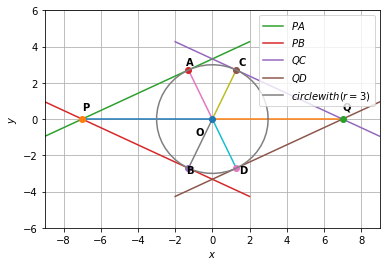
\includegraphics[width=\columnwidth]{FIGURE3.png}
    \caption{Tangent lines to circle of radius 3 units.}
    \label{fig:Tangent lines to circle of radius 3 units.}
\end{figure}    
\end{document}

